\chapter{Grundlagen}
\label{chap:background}

Dieses Kapitel erläutert die Funktionsweise der Sensoren, die für die Methode verwendet werden sowie die wichtigsten Begriffe des maschinellen Lernens, dessen Verständnis für die darauffolgenden Kapitel essentiell ist.

\section{Erläuterung der verwendeten Sensoren}
\label{sec:sensors}
Während in der Einleitung nur generisch von "Sensordaten" die Rede war, werden diese nun konkretisiert. Zur Aufnahme werden das Android-Smartphone OnePlus 3 sowie der Fitness-Tracker Microsoft Band 2 verwendet, der mit dem Smartphone via Bluetooth verbunden ist. Beide Geräte besitzen einen triaxialen Beschleunigungssensor sowie ein triaxiales Gyroskop. Des Weiteren besitzt das Band unter anderem einen Sensor, der den elektrischen Widerstand der Haut des Trägers misst sowie einen Hauttemperatursensor.

\subsection*{Beschleunigungssensor}
\begin{figure}
\centering
\includegraphics[clip=true,trim=0mm 20mm 0mm 20mm, width=0.7\textwidth]{img/accelerometer}
\caption{Illustration des Beschleunigungssensors}
\label{fig:accelerometer}
\end{figure}
Ein Beschleunigungssensor, auch \textit{Accelerometer} genannt, misst die echte Beschleunigung eines Objektes je physikalischer Achse ($x$, $y$ und $z$). Dies beinhaltet auch die Beschleunigung, die von der Erdgravitation ausgeht: Liegt das Objekt beispielsweise auf dem Boden, erfährt es auf der im rechten Winkel zum Boden stehenden Achse eine Beschleunigung von $g \approx 9.81$ $m/s^2$ \cite{SensorsOverview, nistsi}. Über diesen Sensor kann demnach verfolgt werden, wie der Träger sich im Raum bewegt. Abbildung~\ref{fig:accelerometer} illustriert die Sensordaten eines unbewegten Smartphones, dessen Bildschirm parallel zum Boden gehalten wird. \\
Beide Geräte verfügen über einen solchen Sensor.

\subsection*{Gyroskop}
\begin{figure}
\centering
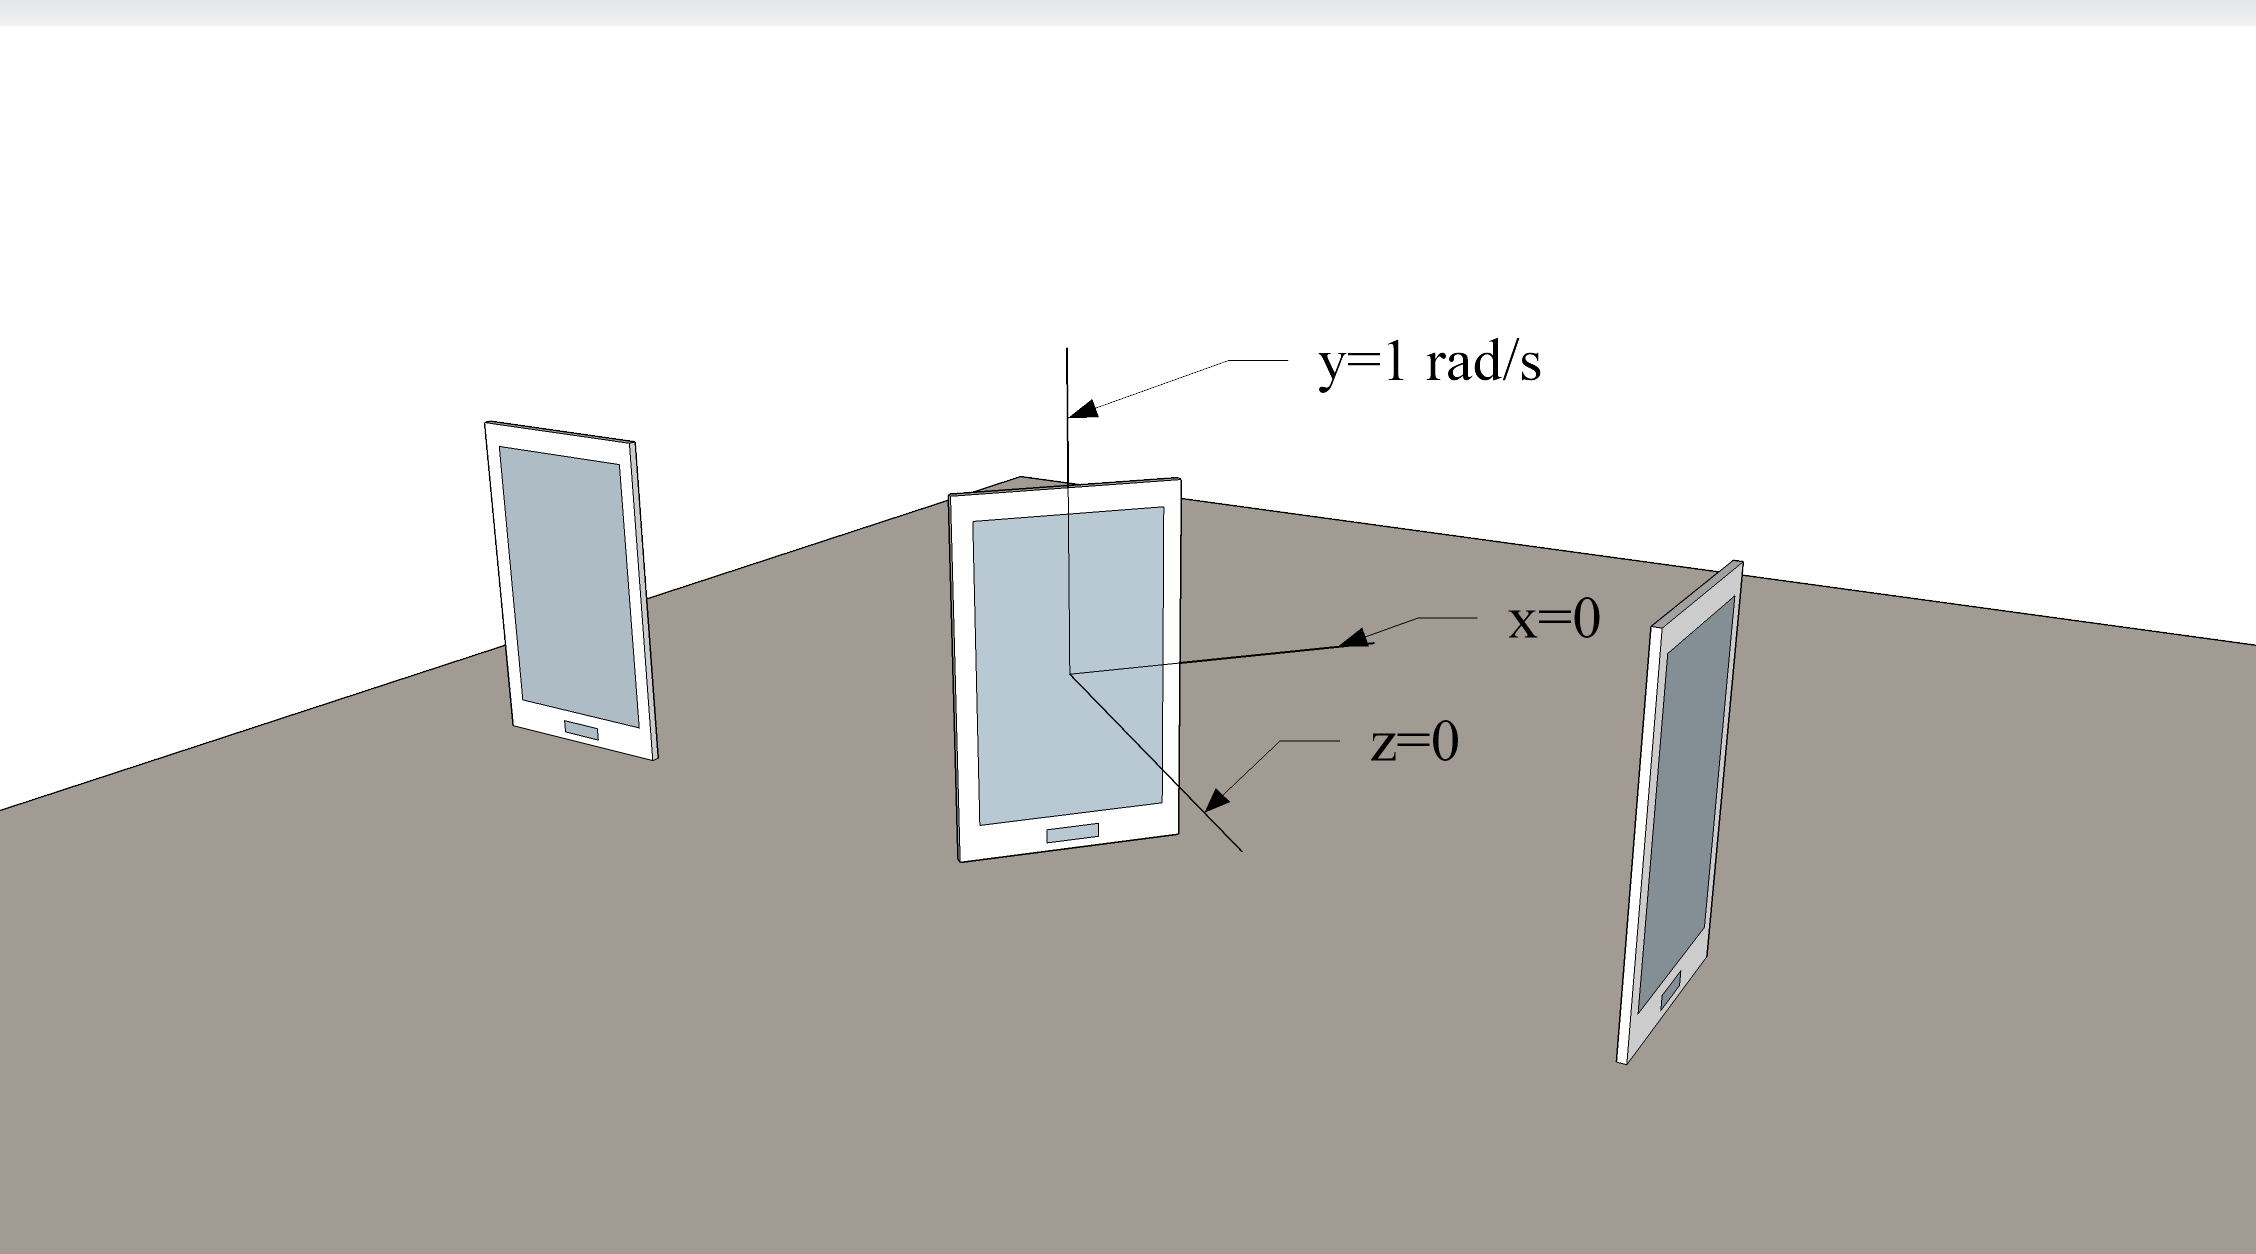
\includegraphics[clip=true,trim=0mm 20mm 0mm 20mm, width=0.7\textwidth]{img/gyroscope}
\caption[Illustration des Gyroskops]{Illustration des Gyroskops. Die Achsenbeschriftungen geben die Rotationsgeschwindigkeit um die jeweilige Achse an. Von links nach rechts wird dasselbe Gerät bei fortschreitender Zeit gezeigt.}
\label{fig:gyroscope}
\end{figure}
Ein Gyroskop, normalerweise Gyrometer genannt, misst die Rotationsgeschwindigkeit je physikalischer Achse \cite{SensorsOverview}. Demnach bedeutet der Messwert $(x=0, y=0, z=0)$, dass das Objekt relativ zur Erde nicht bewegt wird, während $(x=0, y=1, z=0)$ bedeutet, dass das Objekt um die $y$-Achse gedreht wird, wie es beispielhaft in Abbildung~\ref{fig:gyroscope} von links nach rechts gezeigt wird. \\
Beide Geräte verfügen über einen solchen Sensor.

\subsection*{Hautwiderstandssensor}
Je nach aktueller körperlicher Betätigung ändert sich die elektrische Leitfähigkeit der Hautoberfläche durch Schweiß. Der Hautwiderstandssensor misst den elektrischen Widerstand der Haut, der sich umgekehrt proportional zur Leitfähigkeit verhält. Somit können Aussagen über die physische oder psychische Belastung des Trägers getroffen werden.
Dieser Sensor ist nur im Band integriert, das daher für diesen die einzige Datenquelle ist.

\subsection*{Hauttemperatursensor}
Der Hauttemperatursensor misst die Temperatur der Haut des Nutzers, die an der Unterseite des Band anliegt. Leider reagierte dieser Sensor in einem Test nur langsam auf Temperaturveränderungen: Nachdem der Tracker abgelegt wurde, übermittelte dieser den Temperaturabfall erst mehrere Sekunden später. Aus diesem Grund wurde auf die Aufzeichnung dieser Daten verzichtet.

\subsection*{Laufgeschwindigkeitssensor}
Der Laufgeschwindigkeitssensor ist ein virtueller Sensor, der auf Basis des elektronischen Schrittzählers im Microsoft Band 2 generiert wird. Er gibt die geschätzte Laufgeschwindigkeit des Trägers in $cm/s$ an.

\section{Wichtige Begriffe}
In den folgenden Kapiteln wird von einem grundlegenden Verständnis von \ac{ML}-Klassifikation ausgegangen.

\begin{definition}[\ac{ML}-Klassifikation]
\label{def:ml-classification}
Gegeben sei ein Datensatz $D \ni (x_1, ..., x_n, y)$ mit $|D| = m$ Instanzen. Dann sind $x = (x_1, ..., x_n)$ die \textit{Input-Features} und $y$ das \textit{Target}. Im Falle eines Klassifikationsproblems ist $y$ nominal und beschreibt in Form eines Texts eine \textit{Klasse}. Gesucht ist nun eine \textit{Hypothesenfunktion} $h(x) = \hat{y}$, die zu gegebenen Features den wahrscheinlichsten Wert des Targets bestimmt \cite{Ng2011a}.
\end{definition}
Neben Definition~\ref{def:ml-classification} sind für das Verständnis dieser Arbeit die folgenden Begriffe wichtig:
\begin{enumerate}
\item \textit{(Überwachtes) Lernen, bzw. Training} und \textit{Modelle.} Einem \ac{ML}-Algorithmus werden Trainingsdaten $T_1 \subset D$ gezeigt, zu denen das Target bekannt ist. Aus diesem Prozess ergibt sich ein gelerntes \textit{Modell}. 

Weitere Informationen befinden sich in Hastie, Kapitel 2.1 \cite{Hastie2009}.
\item \textit{Overfitting und Train-Test-Split.} Um die Genauigkeit eines Modells zu evaluieren, müssen mit Hilfe dessen Testdaten $T_2 \subset D$ klassifiziert werden, zu denen das Target ebenfalls bekannt ist. Ist $T_1 \cap T_2 \neq \emptyset$, so besteht das Risiko, dass der \ac{ML}-Algorithmus sich den Trainingsdaten zu sehr angepasst hat, daher auch im Test mit $T_2$ genau ist und auf weiteren, noch unbekannten Daten eine schlechte Genauigkeit erzielt (\textit{Overfitting}). 

Weitere Informationen befinden sich in Hastie, Kapitel 7.2 \cite{Hastie2009}.
\item \textit{Kreuzvalidierung.} Bei einer $k$-fachen Kreuzvalidierung werden $k$ Paare $T_1, T_2$ mit $T_1 \cap T_2 = \emptyset$ erstellt, sodass jedes Datum einmal in $T_2$, dann jedoch nicht in $T_1$ enthalten ist. Anschließend wird ein \ac{ML}-Klassifikationsalgorithmus mit jedem $T_1$ trainiert und dem dazugehörigen $T_2$ ausgewertet. 

Weitere Informationen befinden sich in Hastie, Kapitel 7.10 \cite{Hastie2009}.
\item \textit{Hyperparameter.}  Dabei handelt es sich um Parameter eines \ac{ML}-Algorithmus, die dieser nicht eigenständig optimieren kann.
\end{enumerate}

Vor der Entwicklung eines Verfahrens zur Erkennung körperlicher Aktivitäten mittels Smartphone- und Smartwatch-Sensoren und Machine Learning steht die Untersuchung verwandter Arbeiten, die im nächsten Kapitel folgt.

% vim: set ft=tex
